\documentclass[aspectratio=169]{beamer}
\setbeamertemplate{navigation symbols}{}
\usepackage{color,amsmath,comment, subfigure}
\usepackage{booktabs}
\usepackage{url}

%%%%%%%%%%%%%%%%%%%%%%%%%%
\title[]{Lecture 22: Network scale-up method to study groups most at-risk for HIV}
\author[]{Matthew J. Salganik}
\institute[]{Sociology 204: Social Networks\\Princeton University}
\date[]{
2/2 Survey experiment with blending: A network scale-up study in Rwanda
\vfill

\begin{flushleft}
\vspace{0.6in}

\includegraphics[width=0.1\textwidth]{figures/cc.png}
\end{flushleft}
}

\begin{document}
%%%%%%%%%%%%%%%%%%%%%%%%%%%
\frame{\titlepage}
%%%%%%%%%%%%%%%%%%%%%%%%%%%
\begin{frame}

\Large{
\begin{center}
How can we improve\\if we don't know how we are doing?
\end{center}
}

\end{frame}
%%%%%%%%%%%%%%%%%%%%%%%%%%%
\begin{frame}

\begin{center}
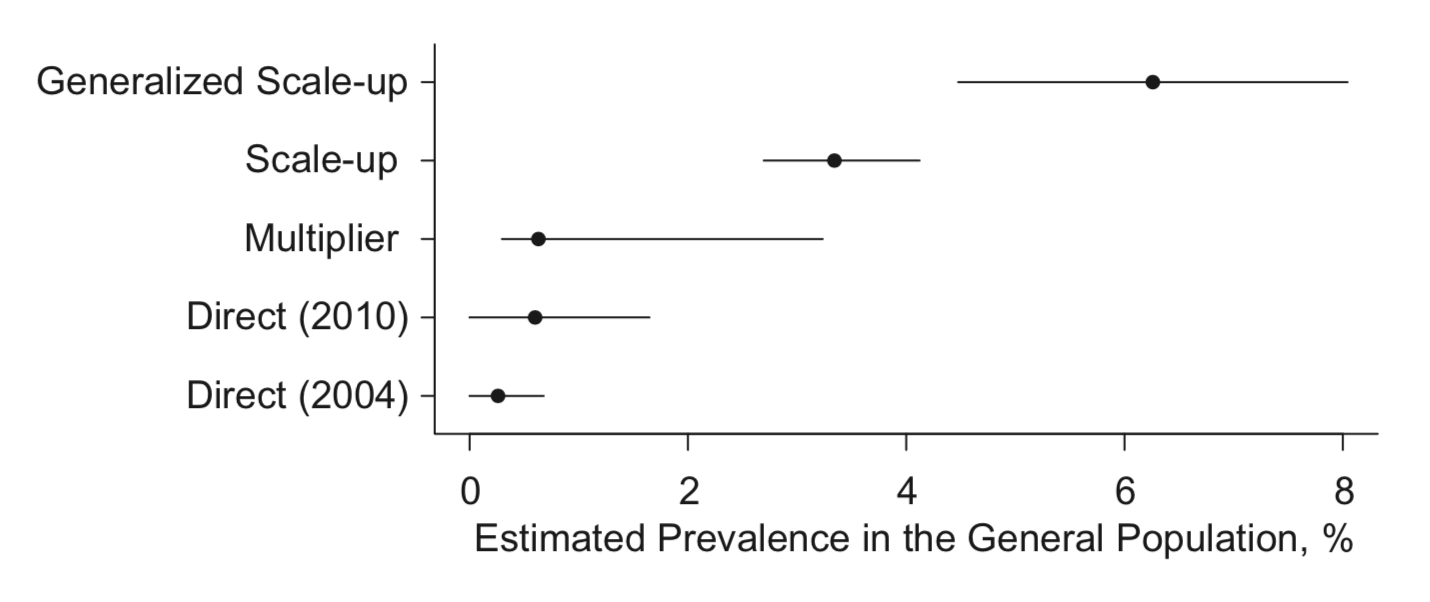
\includegraphics[width=0.9\textwidth]{figures/salganik_assessing_2011_fig2}
\end{center}
\small{
Source: Salganik, M.J., Fazito, D., Bertoni, N., Abdo, A.H., Mello, M.B., and Bastos, F.I. (2011)  \textit{American Journal of Epidemiology}. }

\end{frame}
%%%%%%%%%%%%%%%%%%%%%%%%%%%
\begin{frame}

\begin{center}
How can we reliably make progress in our ability to estimate quantities that will never be known?
\end{center}
\pause
\begin{itemize}
\item Theoretical 
\item Empirical 
\end{itemize}

\note{Theoretical include modeling like we saw in last video}

\end{frame}
%%%%%%%%%%%%%%%%%%%%%%%%%%%
\begin{frame}

\LARGE{Network scale-up study in Rwanda}

\end{frame}
%%%%%%%%%%%%%%%%%%%%%%%%%%%%%%%
\begin{frame}

Study in Rwanda was designed to estimate the number of 
\begin{itemize}
\item men who have sex with men
\item female sex workers
\item clients of female sex workers
\item injection drug users
\end{itemize}

\vfill
AND \\
\vfill
to produce generalizable knowledge about the scale-up method

\end{frame}
%%%%%%%%%%%%%%%%%
\begin{frame}

\begin{center}
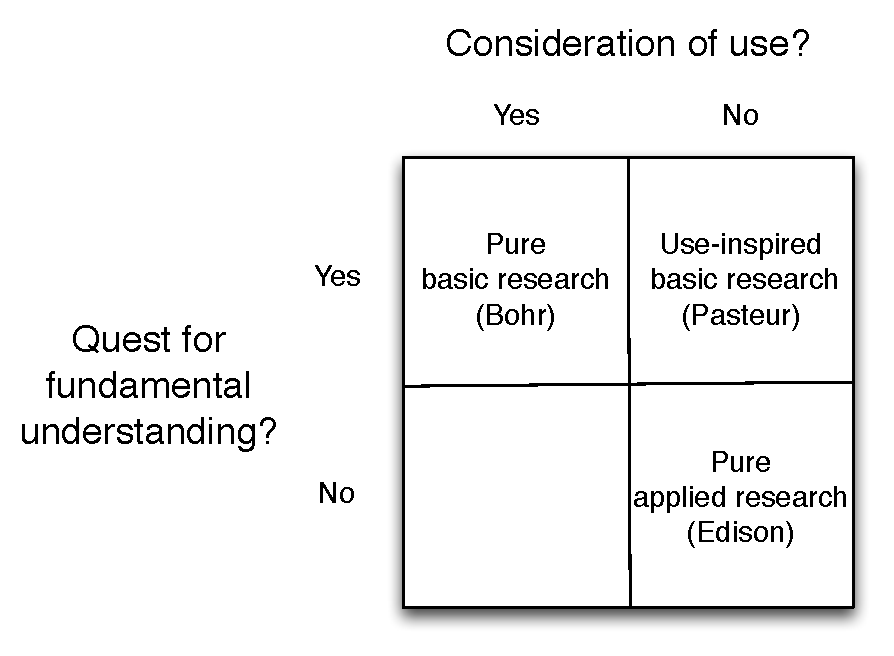
\includegraphics[width=0.6\textwidth]{figures/pasteurs_quadrant}
\end{center}

\end{frame}
%%%%%%%%%%%%%%%%%
\begin{frame}

\begin{itemize}
\item Why was UNAIDS excited about this study?
\pause
\item Why was the Rwandan National AIDS program excited about this study?
\pause
\item Why was I excited about this study?
\end{itemize}

\note{
UNAIDS: methods to be standardized around the world
Rwanda: chance to do more research and learn new methods
Me: advance scale-up and develop template for global use, also inspired by my time at tech companies
}

\end{frame}
%%%%%%%%%%%%%%%%%%%%%%%%%
\begin{frame}

\begin{center}
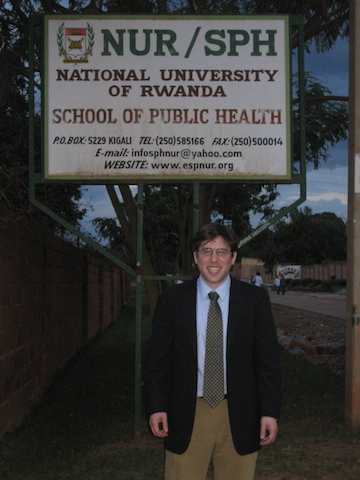
\includegraphics[height=0.9\textheight]{figures/rwanda_matt_nur.jpg}
\end{center}

\end{frame}
%%%%%%%%%%%%%%%%%%%%%%%%%%%%%%
\begin{frame}

\begin{center}
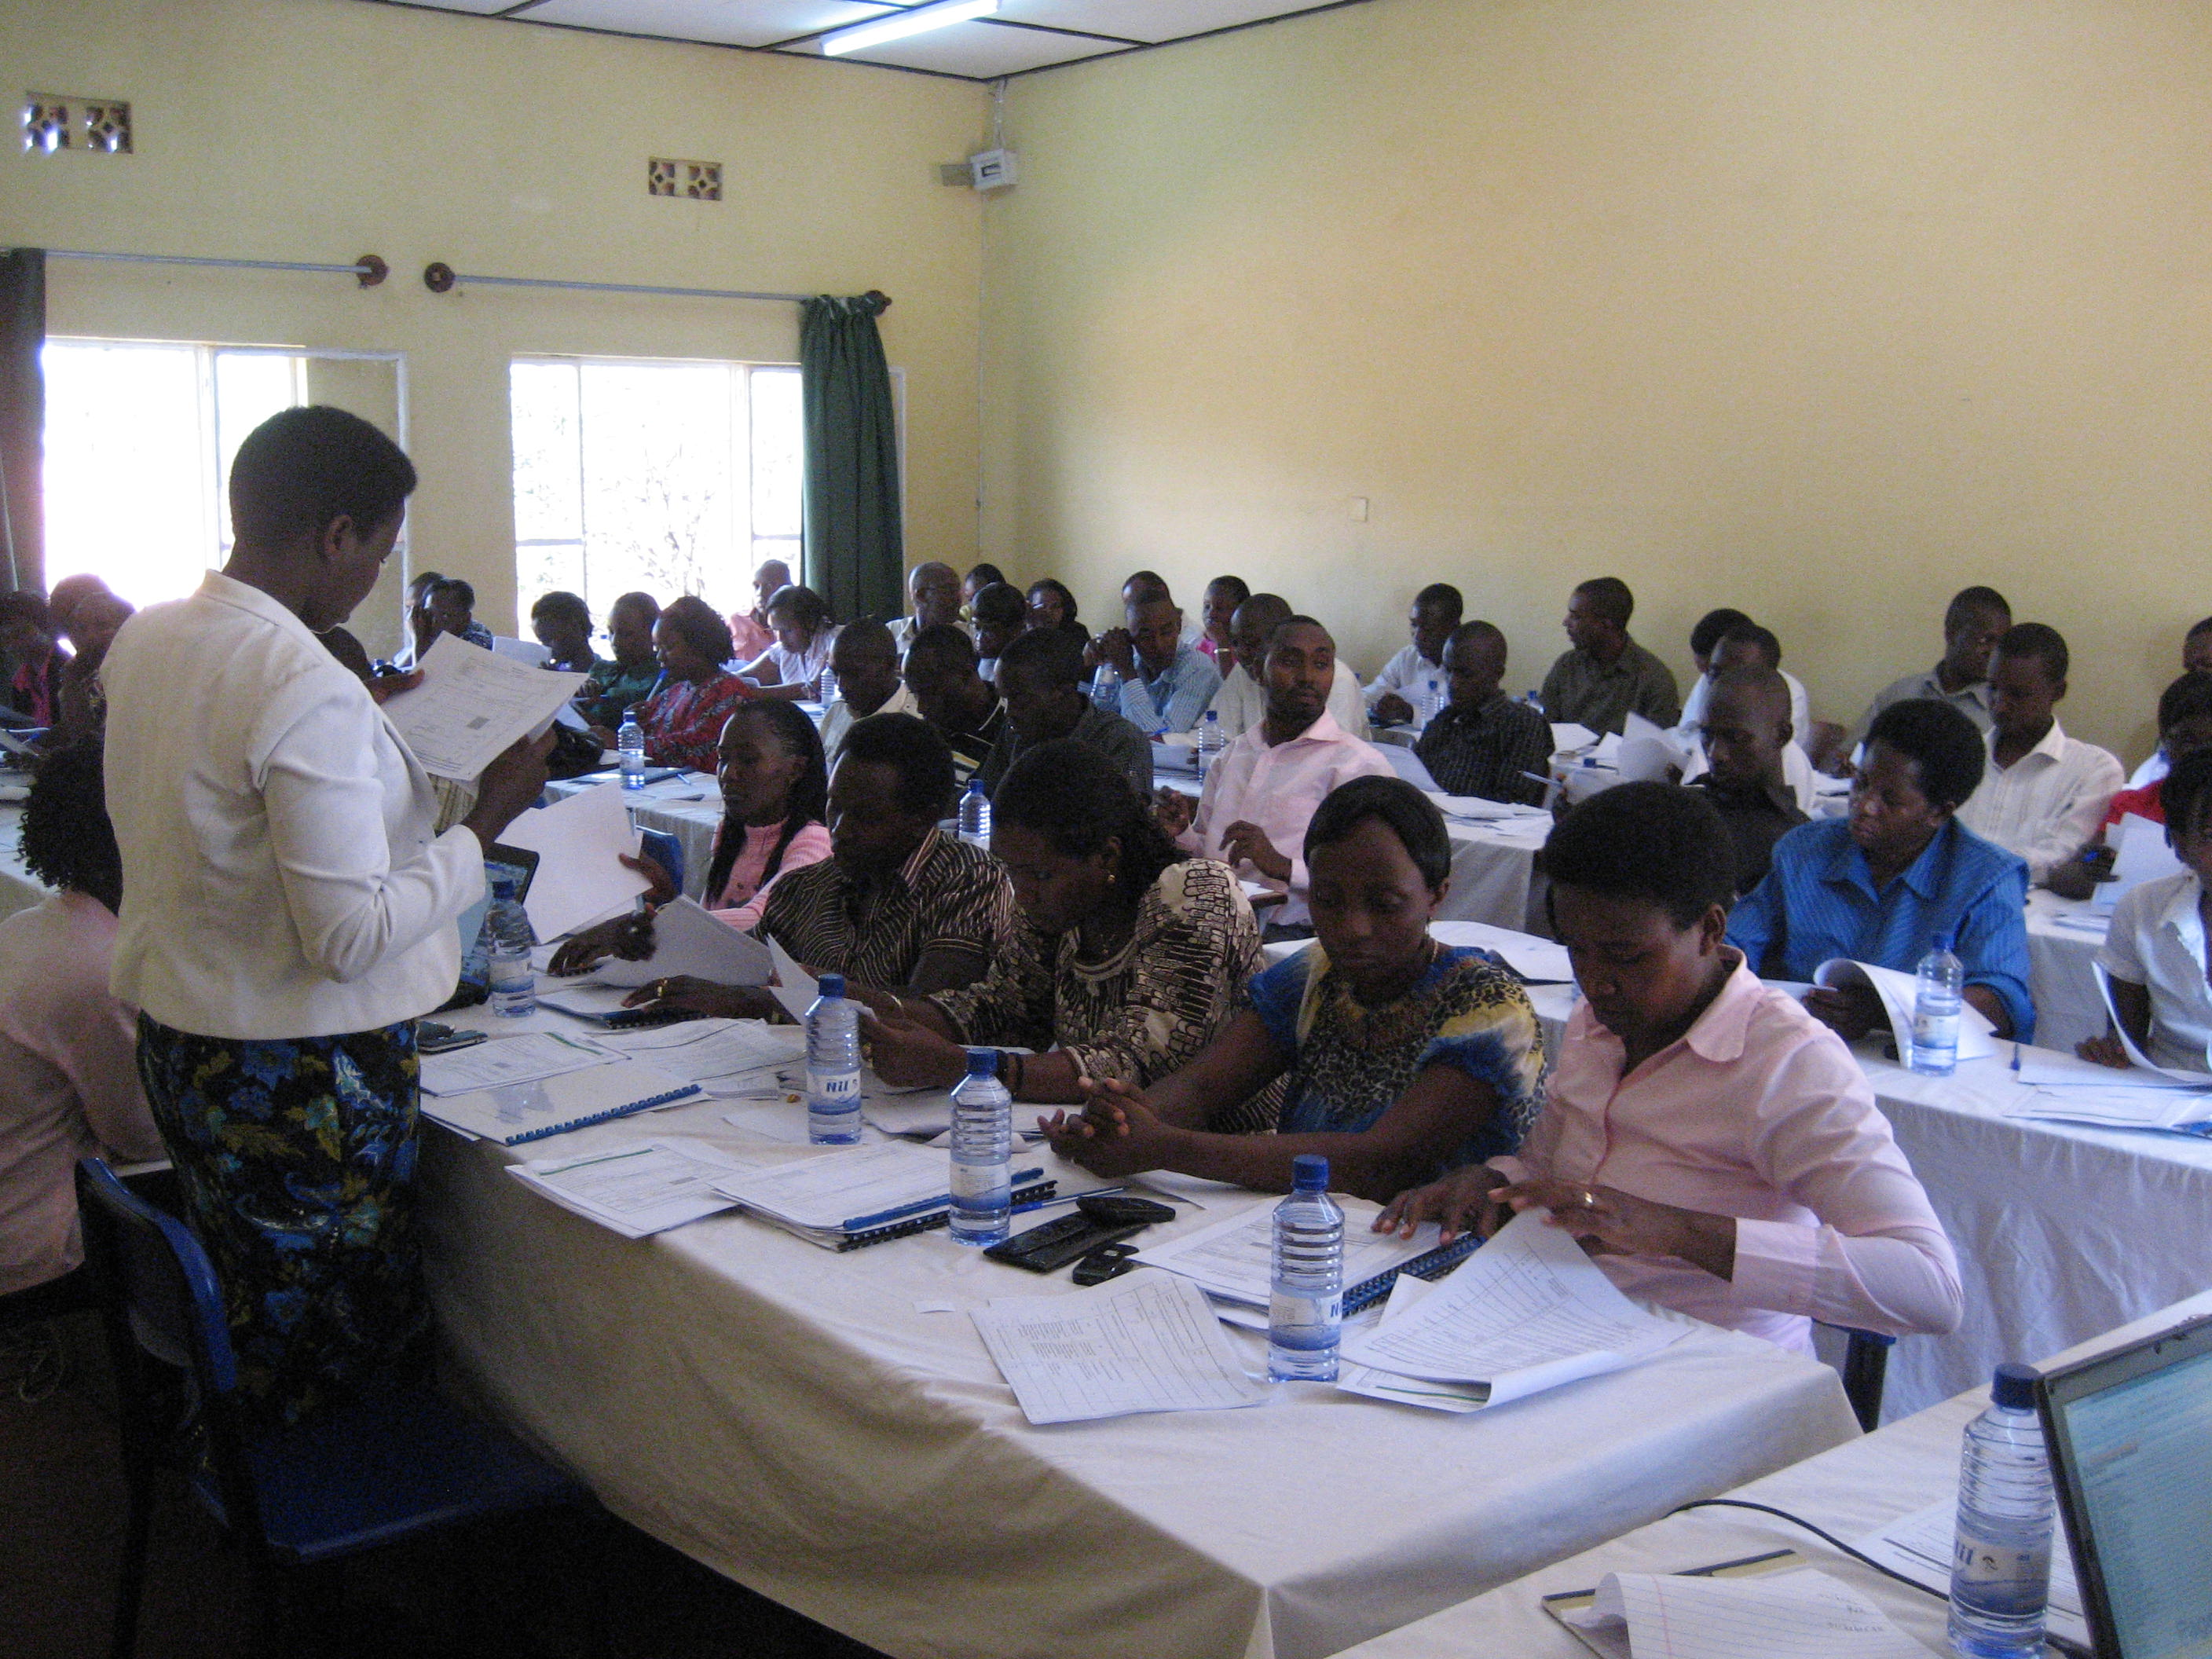
\includegraphics[width=0.8\textwidth]{figures/rwanda_interviewer_class.jpg}
\end{center}

\end{frame}
%%%%%%%%%%%%%%%%%%%%%%%%%%%
\begin{frame}

\begin{center}
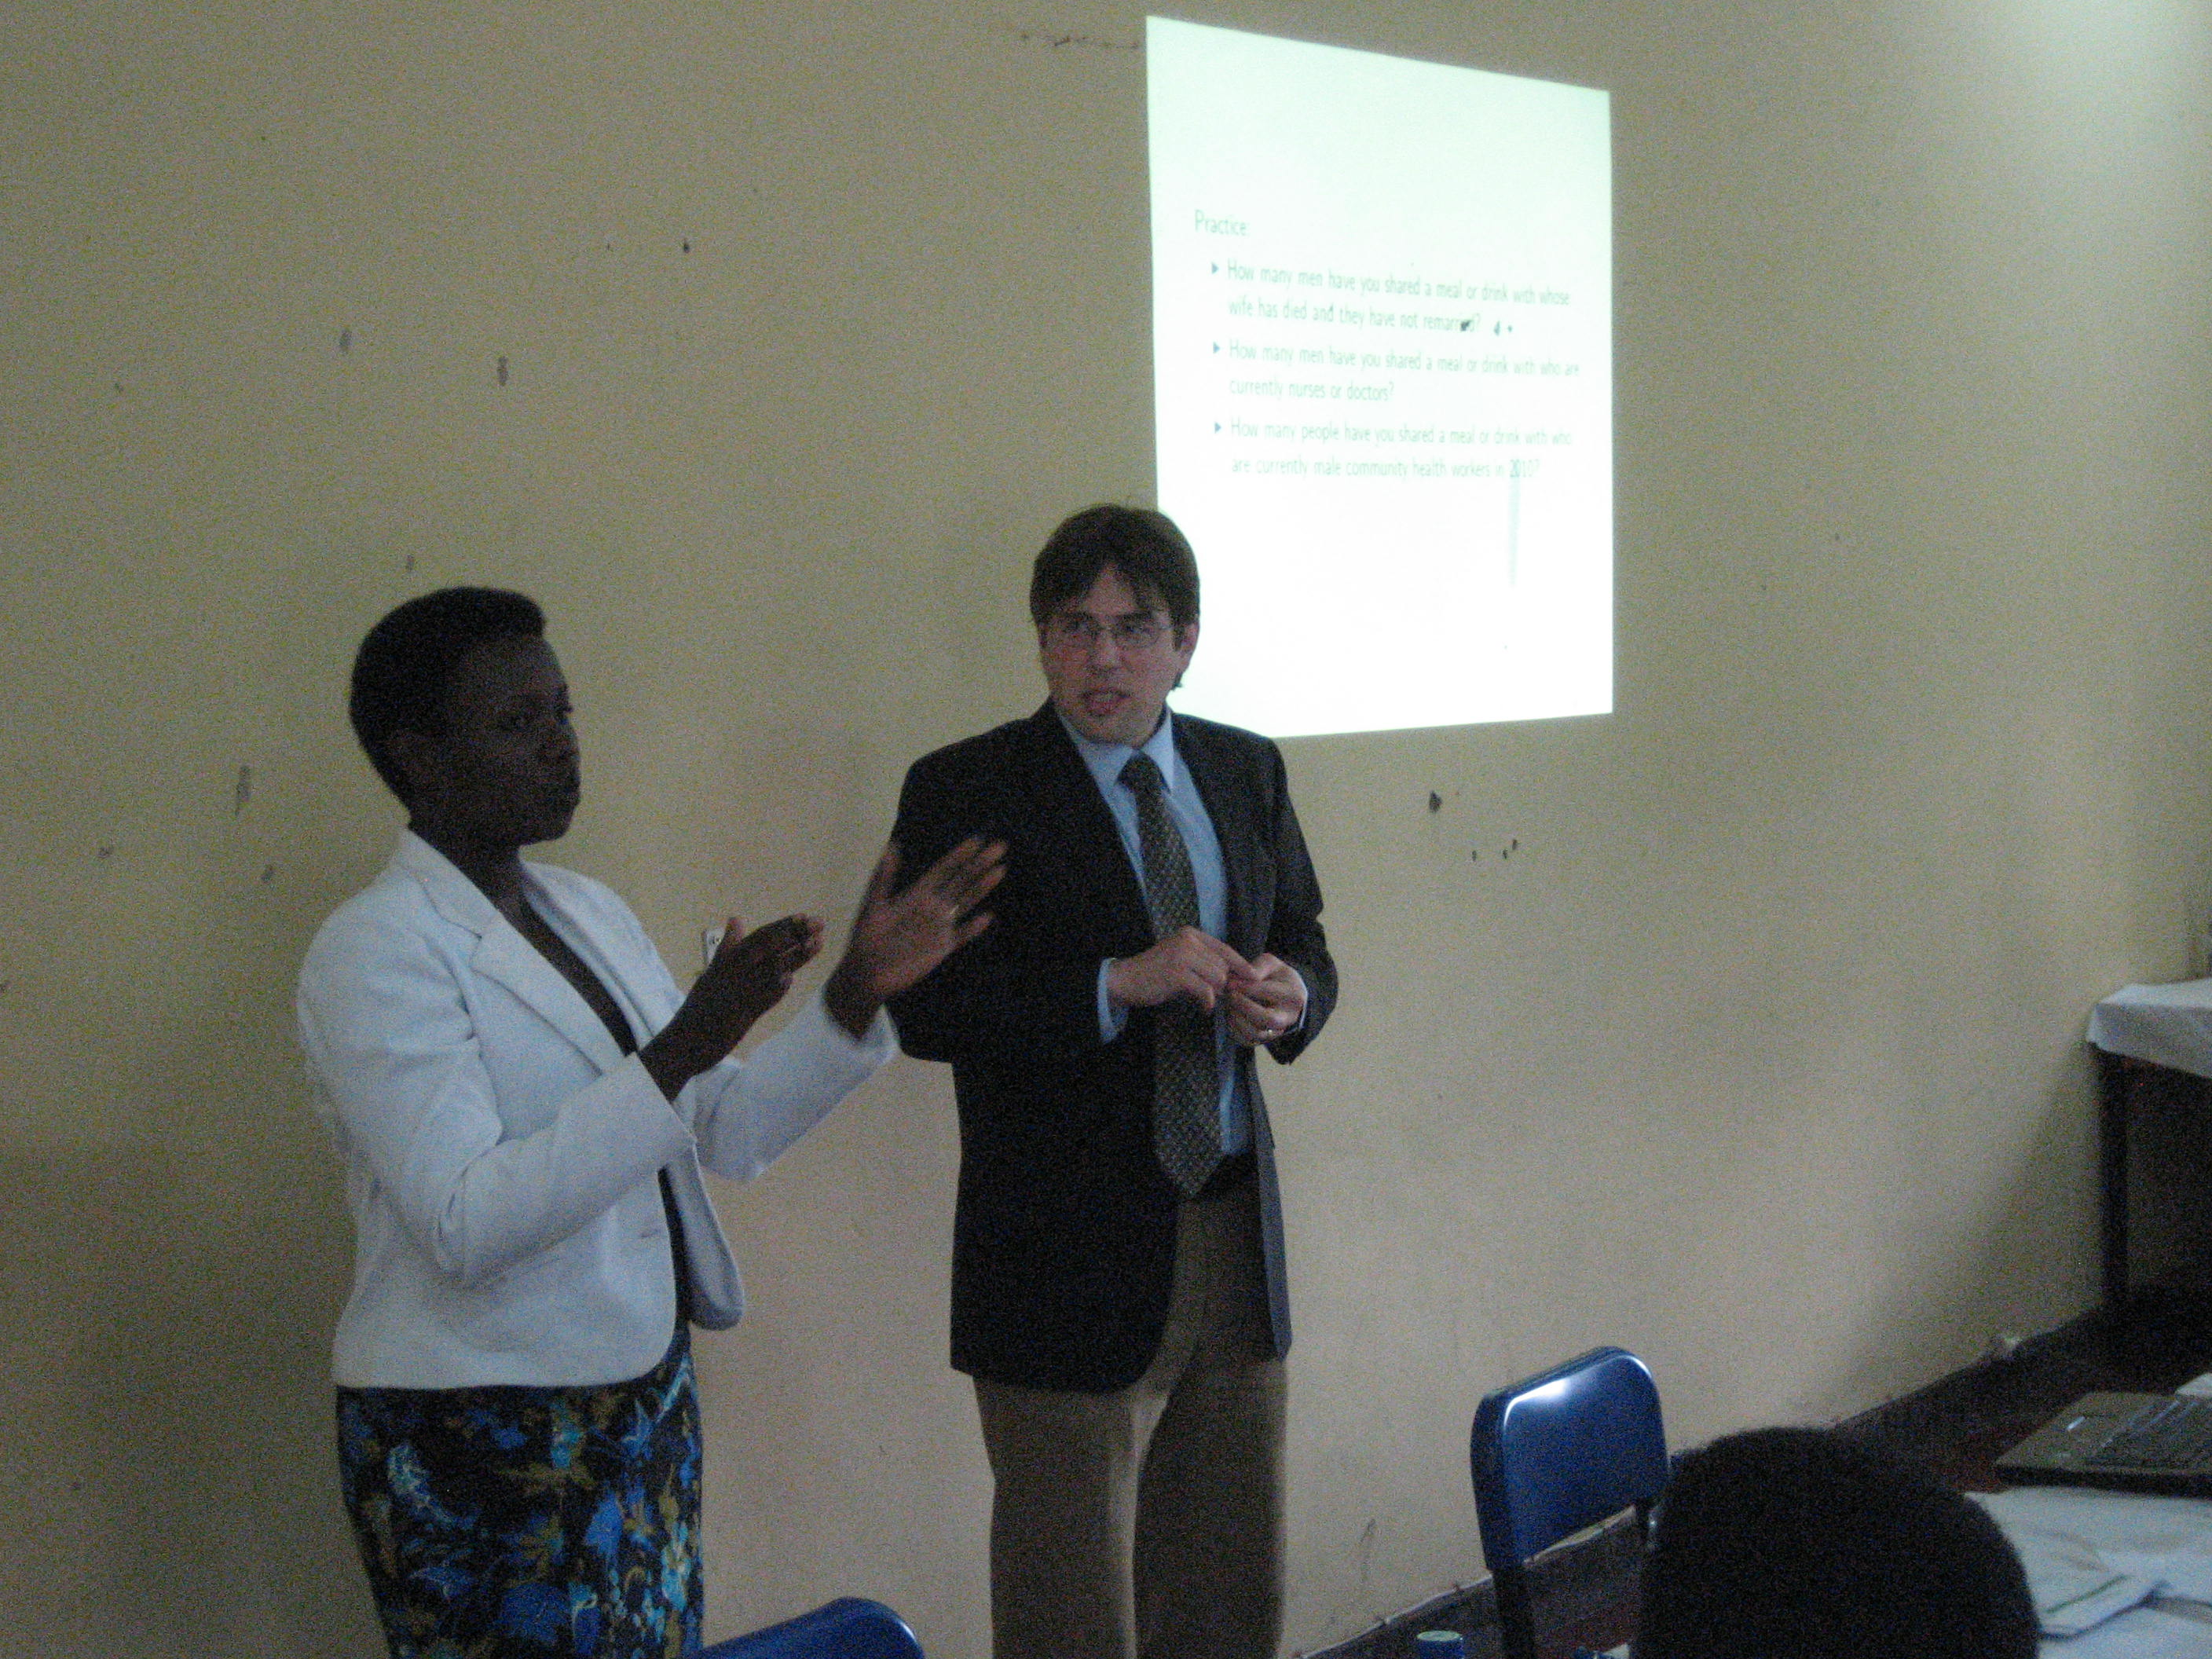
\includegraphics[width=0.8\textwidth]{figures/rwanda_matt_teaching.jpg}
\end{center}

\end{frame}
%%%%%%%%%%%%%%%%%%%%%%%%%%%
\begin{frame}

\begin{center}
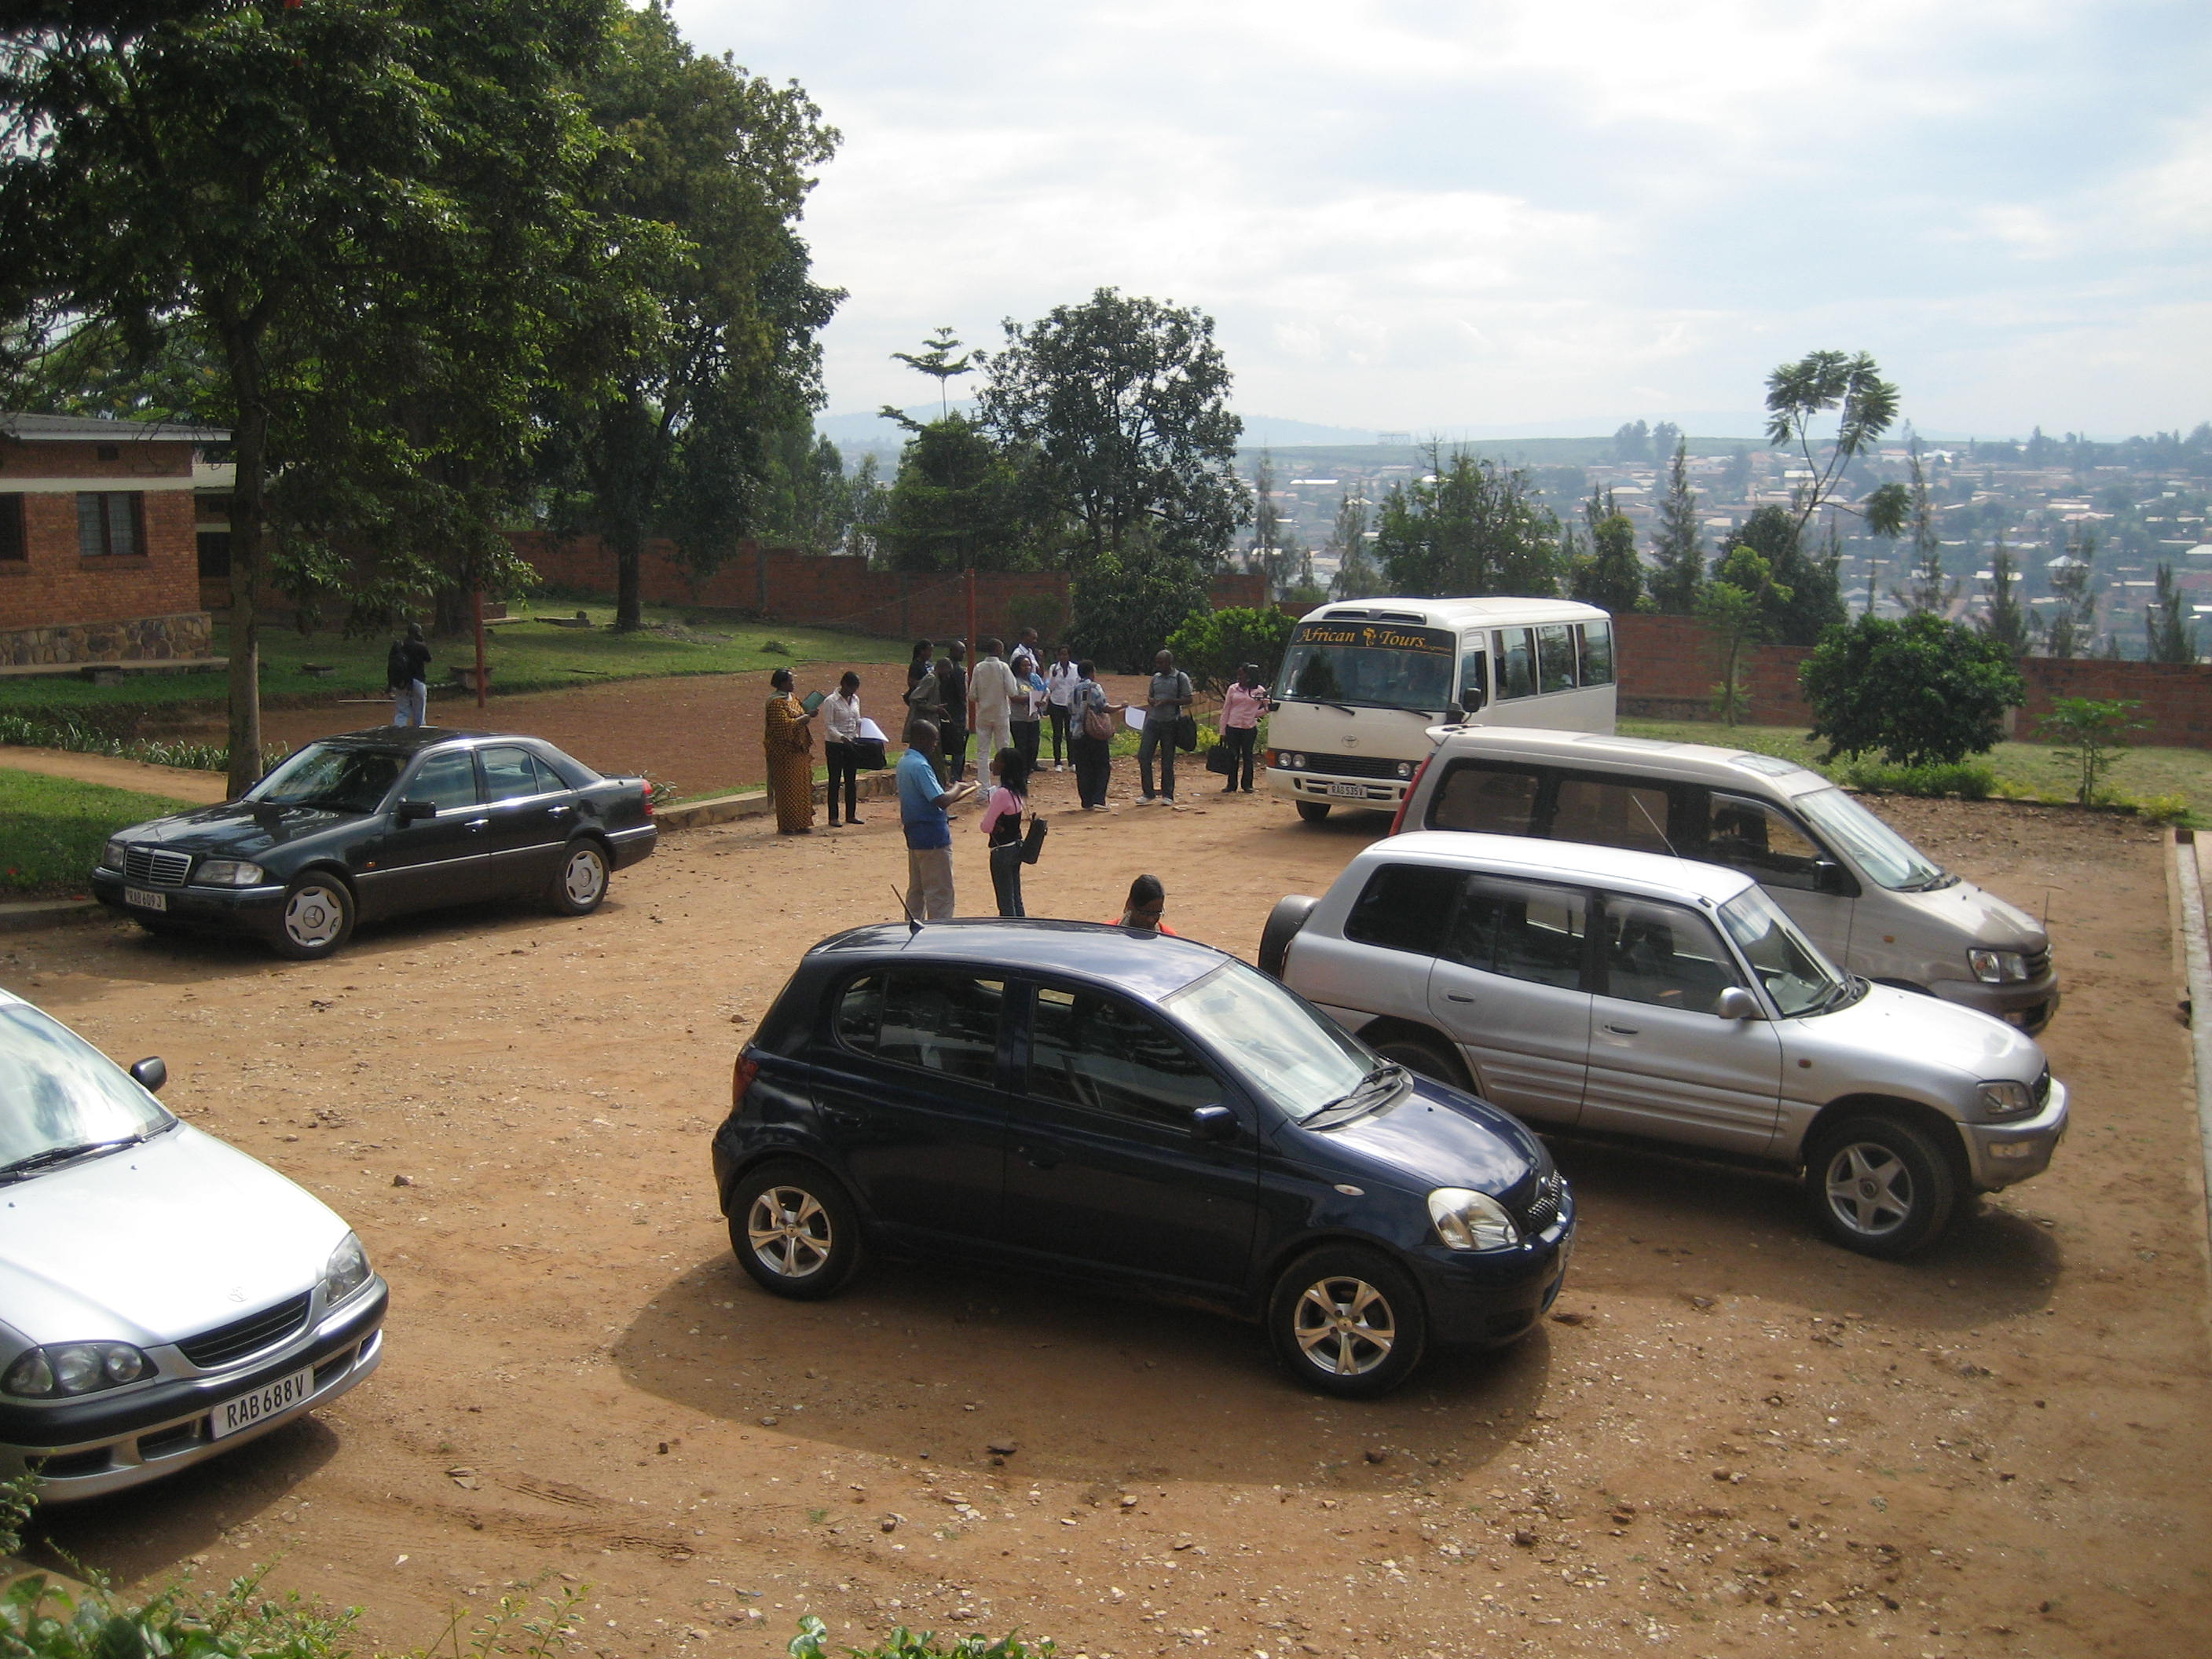
\includegraphics[width=0.8\textwidth]{figures/rwanda_interviewer_bus.jpg}
\end{center}

\end{frame}
%%%%%%%%%%%%%%%%%%%%%%%%%%%
\begin{frame}

\begin{center}
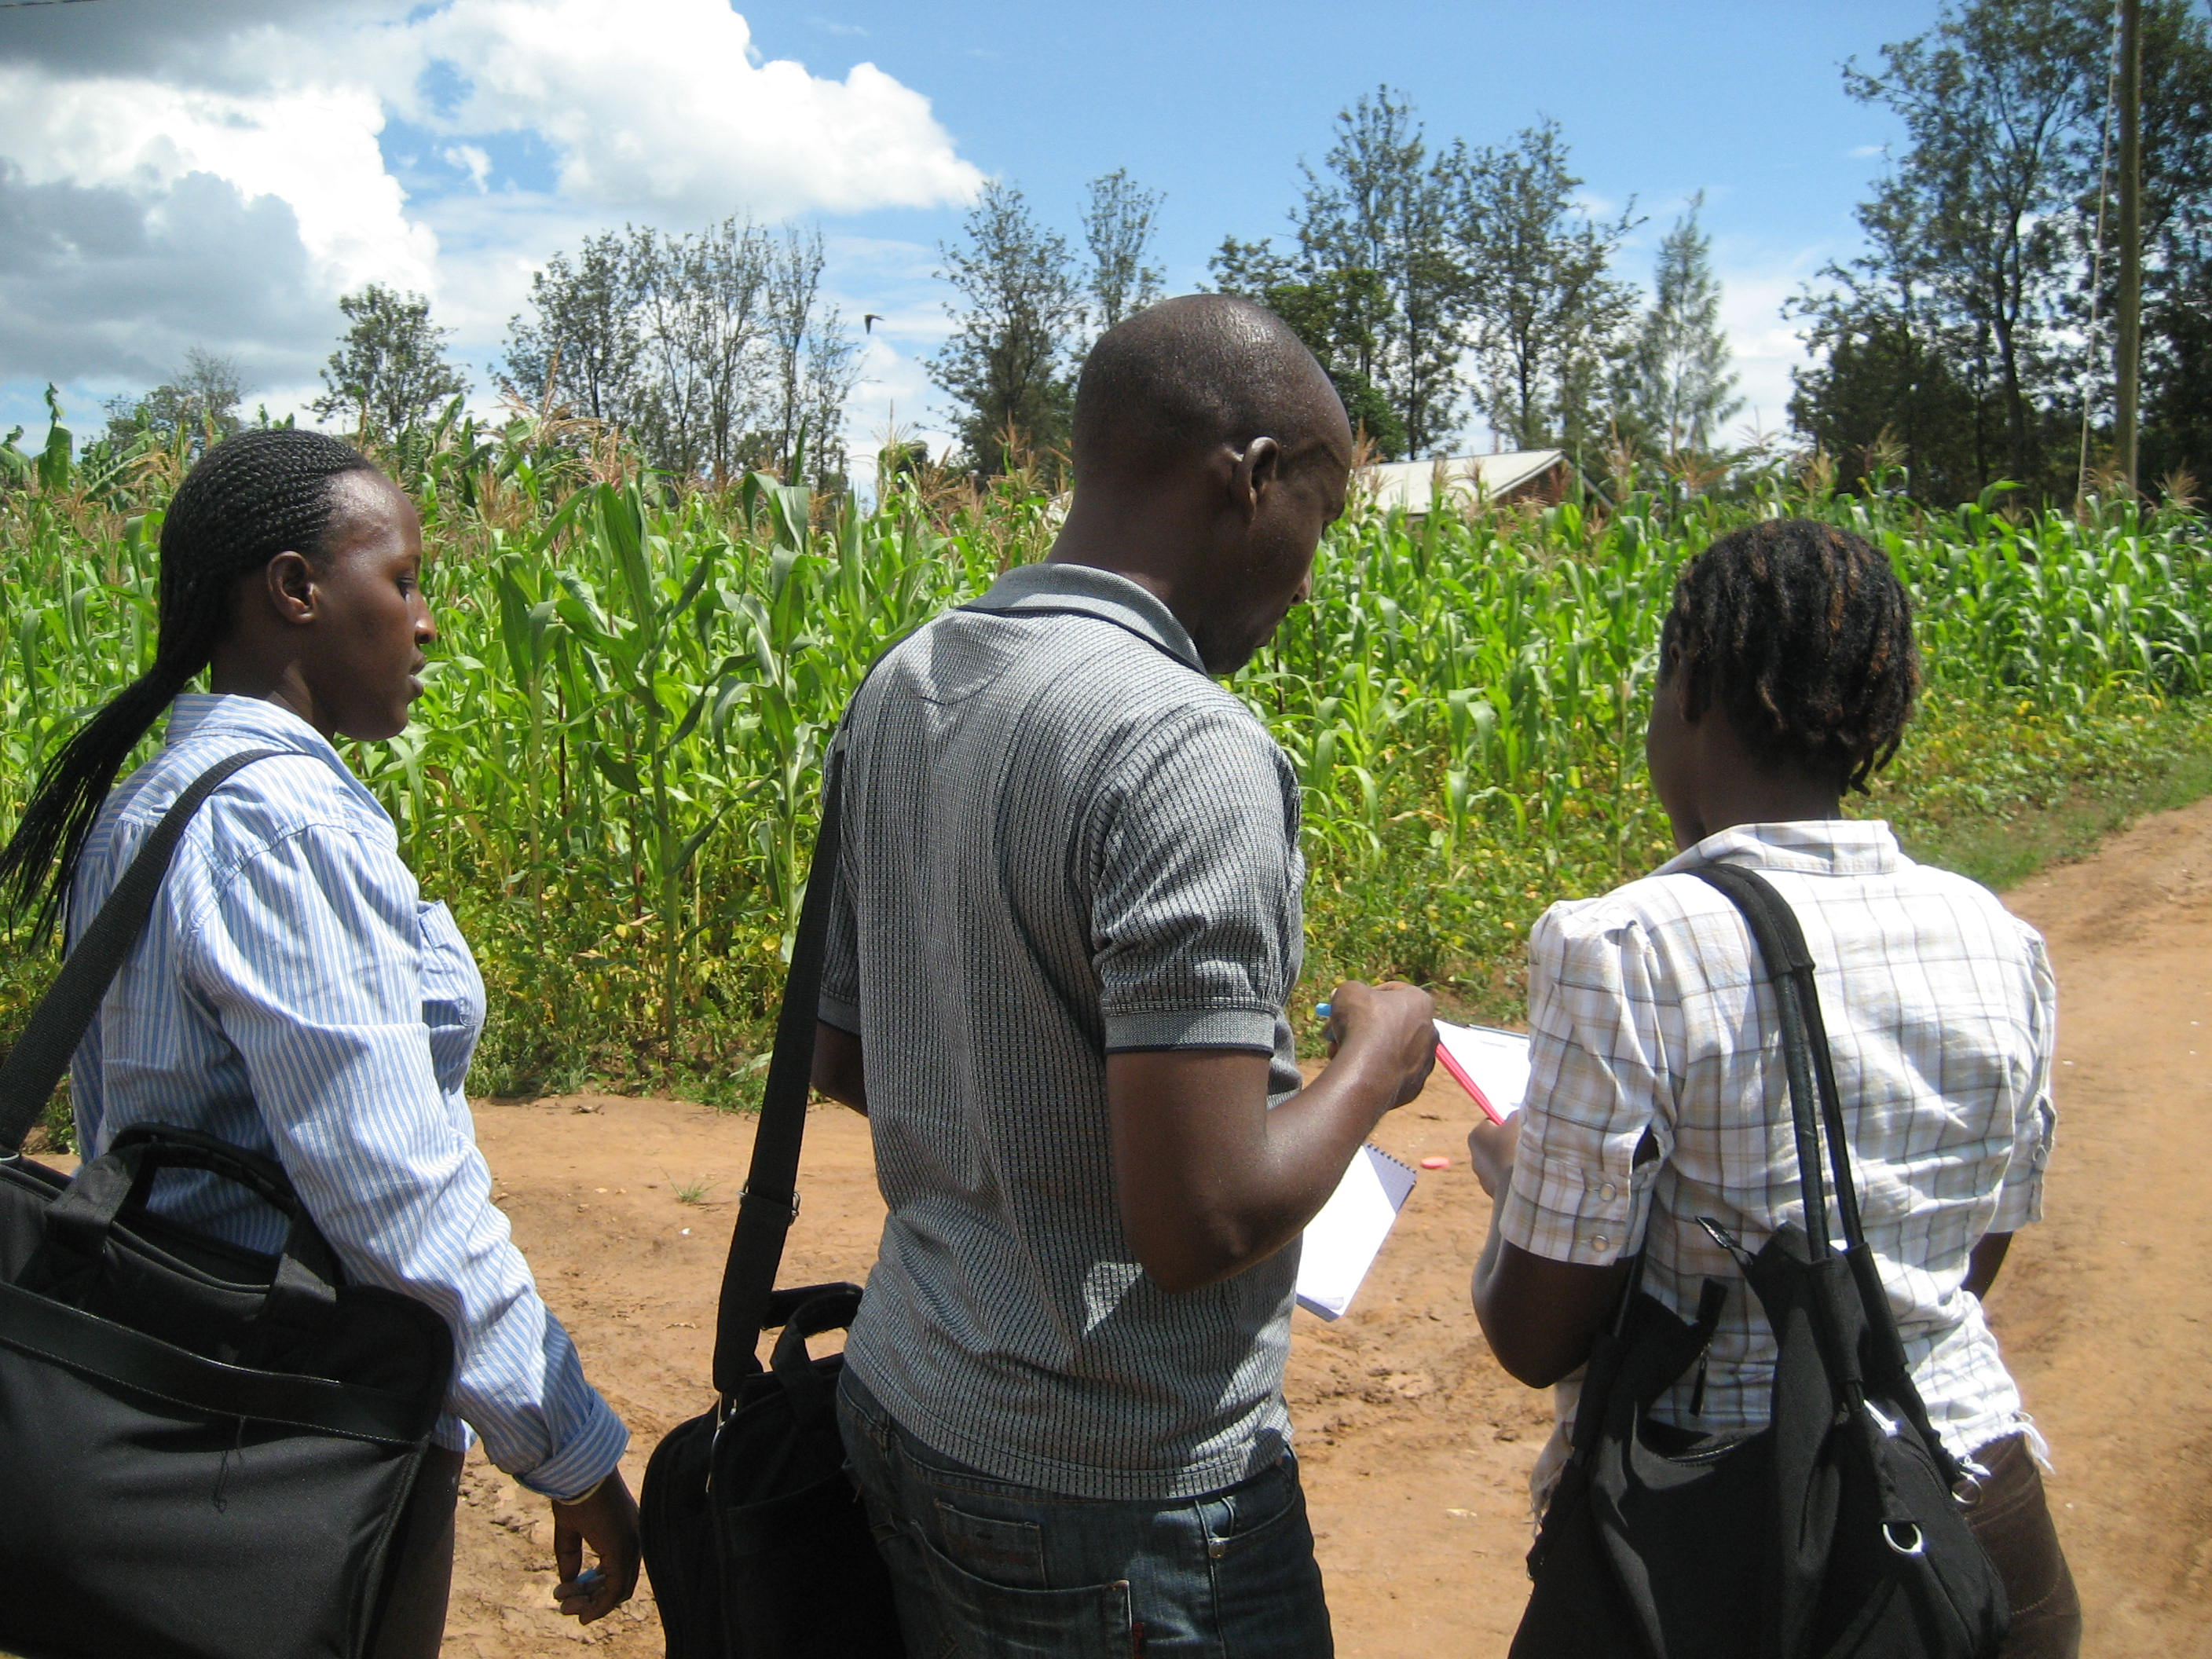
\includegraphics[width=0.8\textwidth]{figures/rwanda_fieldwork.jpg}
\end{center}

\end{frame}
%%%%%%%%%%%%%%%%%%%%%%%%%%%
\begin{frame}

\begin{center}
\includegraphics<1>[width=0.7\textwidth]{figures/tie_strength_axes}
\includegraphics<2>[width=0.7\textwidth]{figures/tie_strength_sampling}
\includegraphics<3>[width=0.7\textwidth]{figures/tie_strength_sampling_non_sampling}
\includegraphics<4>[width=0.7\textwidth]{figures/tie_strength_sampling_non_sampling_total}
\includegraphics<5>[width=0.7\textwidth]{figures/tie_strength_total}
\end{center}

\note{Think back to Granovetter}

\end{frame}
%%%%%%%%%%%%%%%%%%%%%%%%%%%
\begin{frame}
\frametitle{}

{\Large
\begin{center}
\textcolor{blue}{Basic definition} ($n=2,500$)
\end{center}
}
\begin{itemize}
\item people you know by sight and name and who also know you by sight and name  
\item people you have \textcolor{blue}{had some contact with} in the past 12 months
\item people of all ages who live in Rwanda
\end{itemize}

{\Large
\begin{center}
\textcolor{red}{Meal definition} ($n=2,500$)
\end{center}
}
\begin{itemize}
\item people you know by sight and name and who also know you by sight and name  
\item people you have \textcolor{red}{shared a meal or drink with} in the past 12 months
\item people of all ages who live in Rwanda
\end{itemize}

\end{frame}
%%%%%%%%%%%%%%%
\begin{frame}

\begin{columns}
\column{0.5\textwidth}
\begin{center}
\begin{tabular}{l}
\toprule
Priests\\
Nurses or Doctors\\
Male Community Health Worker\\
Widowers\\
Teachers\\
Divorced Men\\
Incarcerated people\\
Women who smoke\\
Muslim\\
Women who gave birth in the last 12 mo.\\
\bottomrule
\end{tabular}
\end{center}

\column{0.5\textwidth}
\begin{center}
\begin{tabular}{l}
\toprule
Twahirwa\\
Mukandekezi\\
Nyiraneza\\
Ndayambaje\\
Murekatete\\
Nsengimana\\
Mukandayisenga\\
Ndagijimana\\
Bizimana\\
Nyirahabimana\\
Nsabimana\\
Mukamana\\
\bottomrule
\end{tabular}
\end{center}

\end{columns}

\end{frame}
%%%%%%%%%%%%%%%
\begin{frame}

\begin{center}
\includegraphics<1>[width=0.6\textwidth]{figures/rwanda_mean_reported_ties}
\end{center}

\end{frame}
%%%%%%%%%%%%%%%
\begin{frame}

\begin{center}
\includegraphics<1>[width=0.8\textwidth]{figures/feehan_quantity_2016_fig2}
\end{center}

\end{frame}
%%%%%%%%%%%%%%%
\begin{frame}

\begin{center}
\includegraphics<1>[width=0.8\textwidth]{figures/rwanda_iv_results}
\end{center}

\begin{center}
Meal definition has lower error (RMSE, MAE, MRE)
\end{center}

\end{frame}
%%%%%%%%%%%%%%%
\begin{comment}
\begin{frame}

\begin{center}
Meal definition has lower error than basic definition
\end{center}
\vfill
\includegraphics<1>[width=\textwidth]{figures/rwanda_error_metrics}

\end{frame}
\end{comment}
%%%%%%%%%%%%%%%
\begin{frame}

\begin{center}
\includegraphics<1>[width=0.8\textwidth]{figures/rwanda_estimates_noblended}
\end{center}

\end{frame}
%%%%%%%%%%%%%%%
\begin{frame}

\begin{equation*}
\hat{N}_H  = w \cdot \hat{N}_{H [meal]} + (1 - w) \cdot \hat{N}_{H [basic]}
\end{equation*}
\pause
\vfill
\begin{equation*}
w = \frac{\widehat{\sigma}^2_{basic}}{\widehat{\sigma}^2_{basic} + \widehat{\sigma}^2_{meal}} 
\end{equation*}

\end{frame}
%%%%%%%%%%%%%%%
\begin{frame}

\begin{center}
\includegraphics<1>[width=\textwidth]{figures/rwanda_estimates_blended}
\end{center}

\end{frame}
%%%%%%%%%%%%%%%
\begin{frame}

\begin{equation*}
N_H = \alpha \hat{N}_H
\end{equation*}

where
\begin{equation*}
\alpha =  \underbrace{\left( \frac{\eta_F}{\tau_F} \right)}_{\text{reporting  distortions}} \times \underbrace{\left( \frac{1}{\phi_F \delta_F} \right)}_{\text{structural distortions}}
\end{equation*}

\end{frame}
%%%%%%%%%%%%%%%
\begin{frame}

\begin{center}
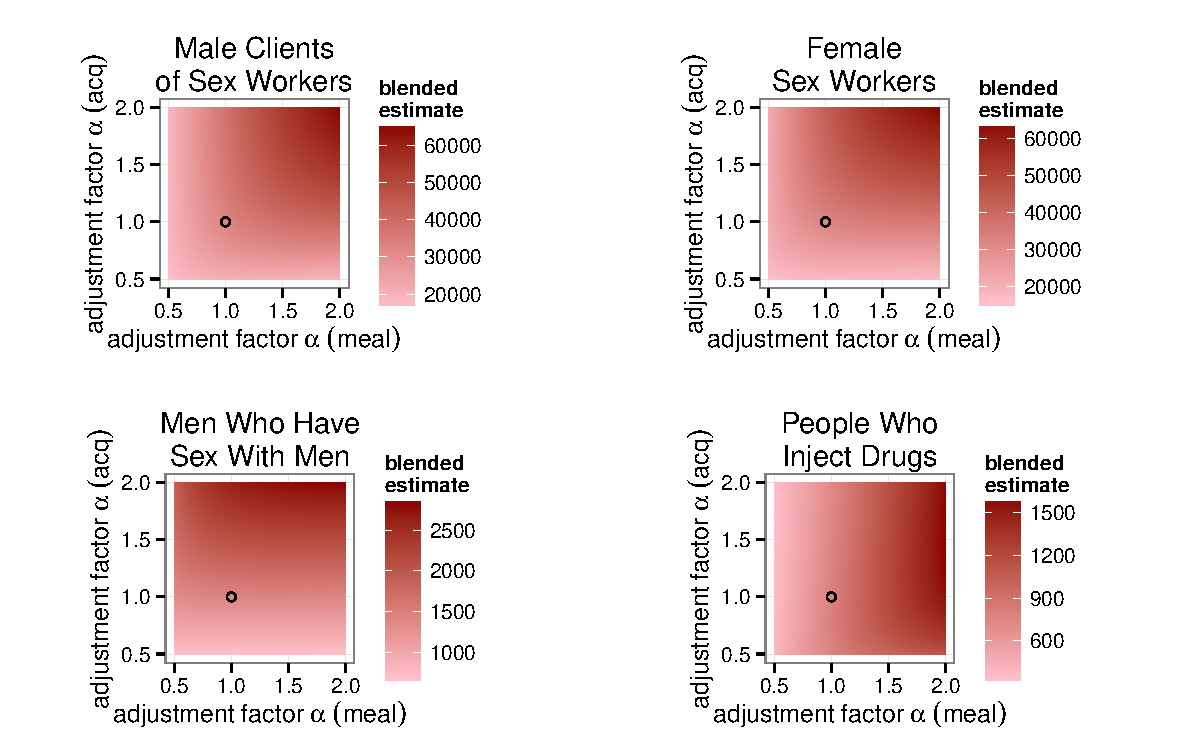
\includegraphics[width=\textwidth]{figures/feehan_quality_fig6}
\end{center}

\end{frame}
%%%%%%%%%%%%%%%
\begin{frame}

\begin{center}
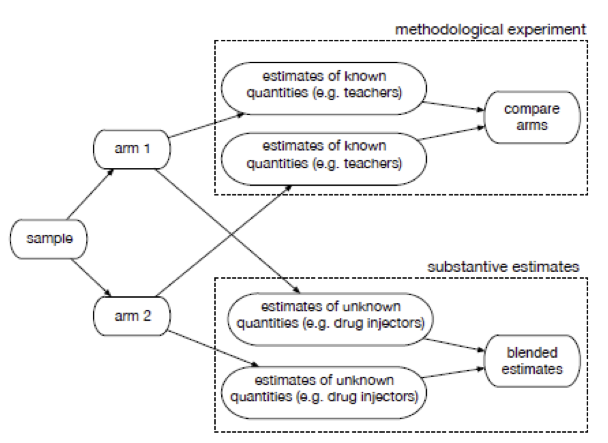
\includegraphics[width=0.8\textwidth]{figures/feehan_quality_2015_fig7}
\end{center}

\end{frame}
%%%%%%%%%%%%%%%%%%%%%%%%%%%
\begin{frame}

\LARGE{Extensions}

\end{frame}
%%%%%%%%%%%%%%%%%%%%%%%%%%%
\begin{frame}

With only two arms, we cannot demonstrate U-shaped relationship!

\begin{center}
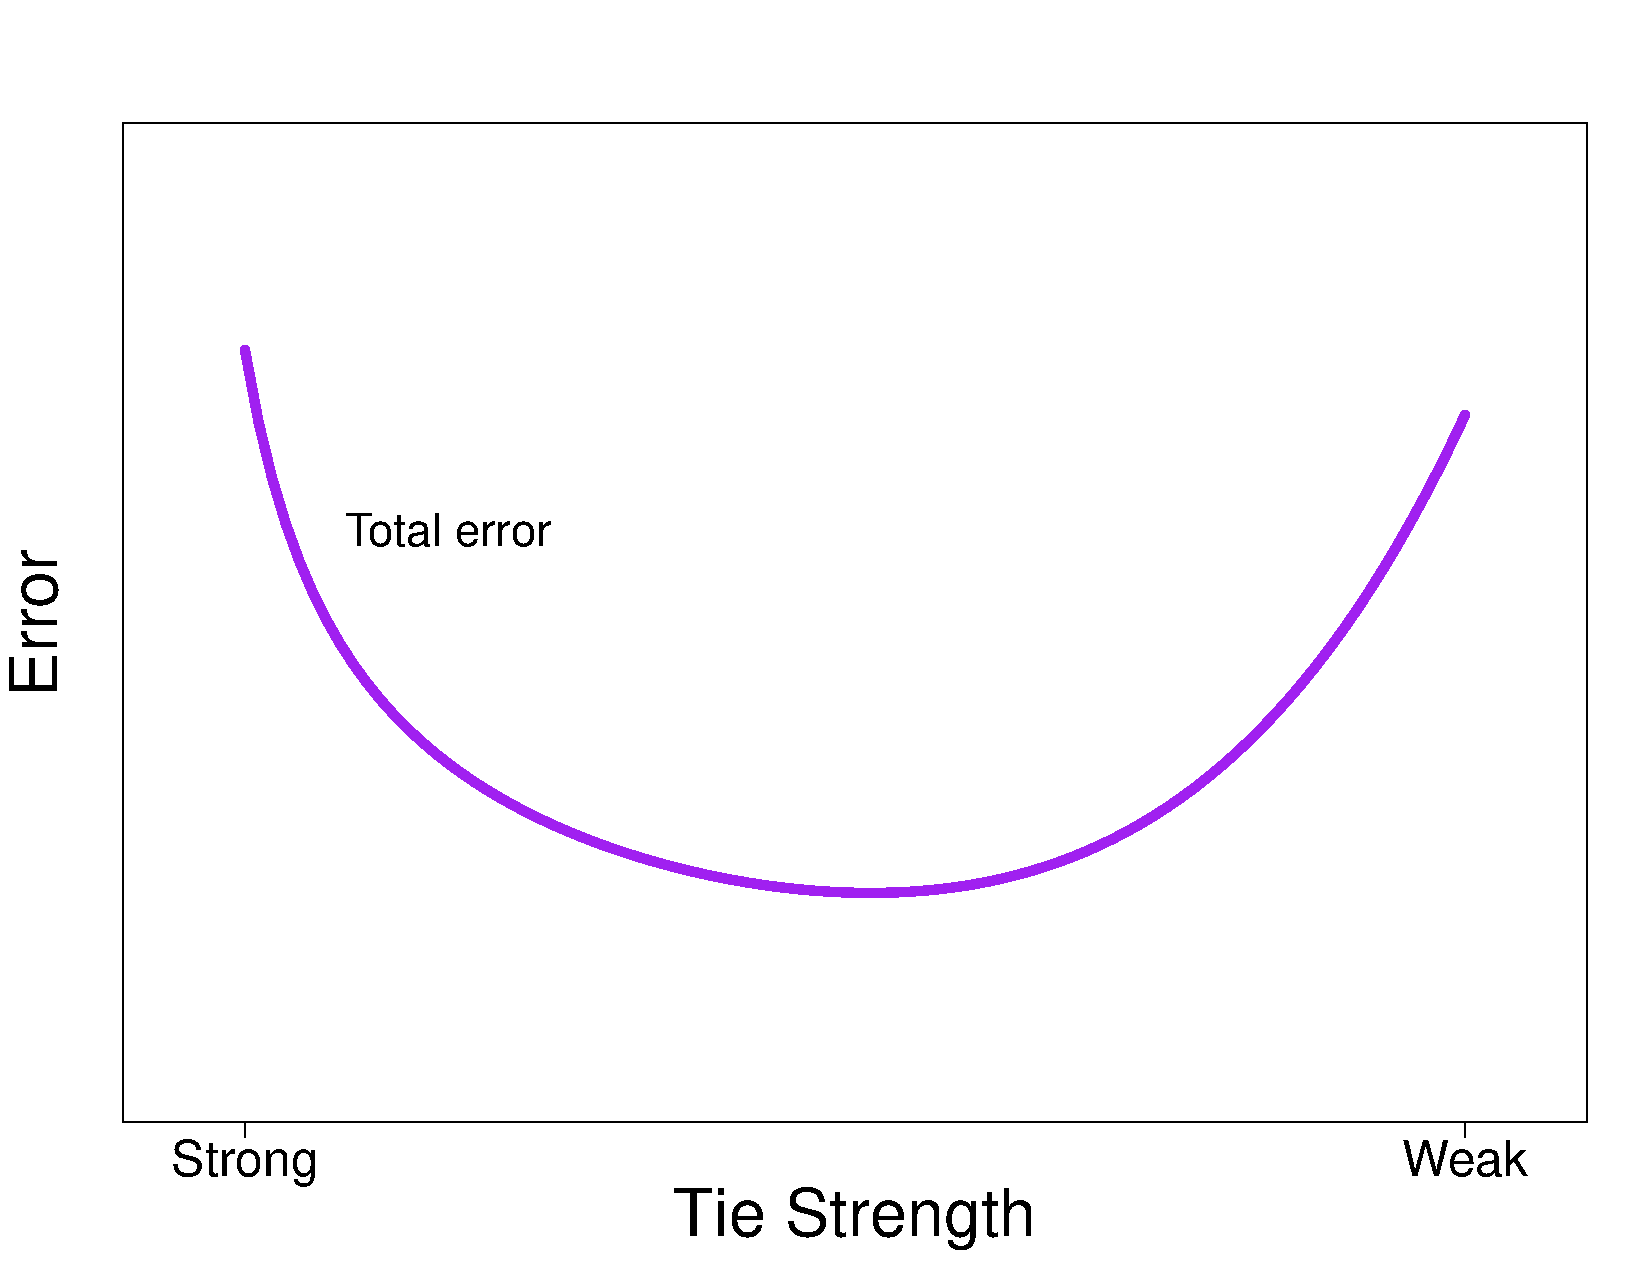
\includegraphics[width=0.25\textwidth]{figures/tie_strength_total}
\end{center}

\pause
In previous classes, we tried a survey experiment as a homework assignment in this class.  
\begin{itemize}
\item We wanted to estimate number of people dating someone from their high school and number of people dating someone from Rutgers.
\item We asked about connections to 9 groups of known size (e.g., sociology majors).
\item We used 4 definitions of to know:
\begin{enumerate}
\item shared a meal with yesterday
\item shared a meal with in the past seven days
\item shared a meal with this semester
\item shared a meal with this academic year
\end{enumerate}
\end{itemize}

\end{frame}
%%%%%%%%%%%%%%%%%%%%%%%%%%
\begin{frame}

\begin{center}
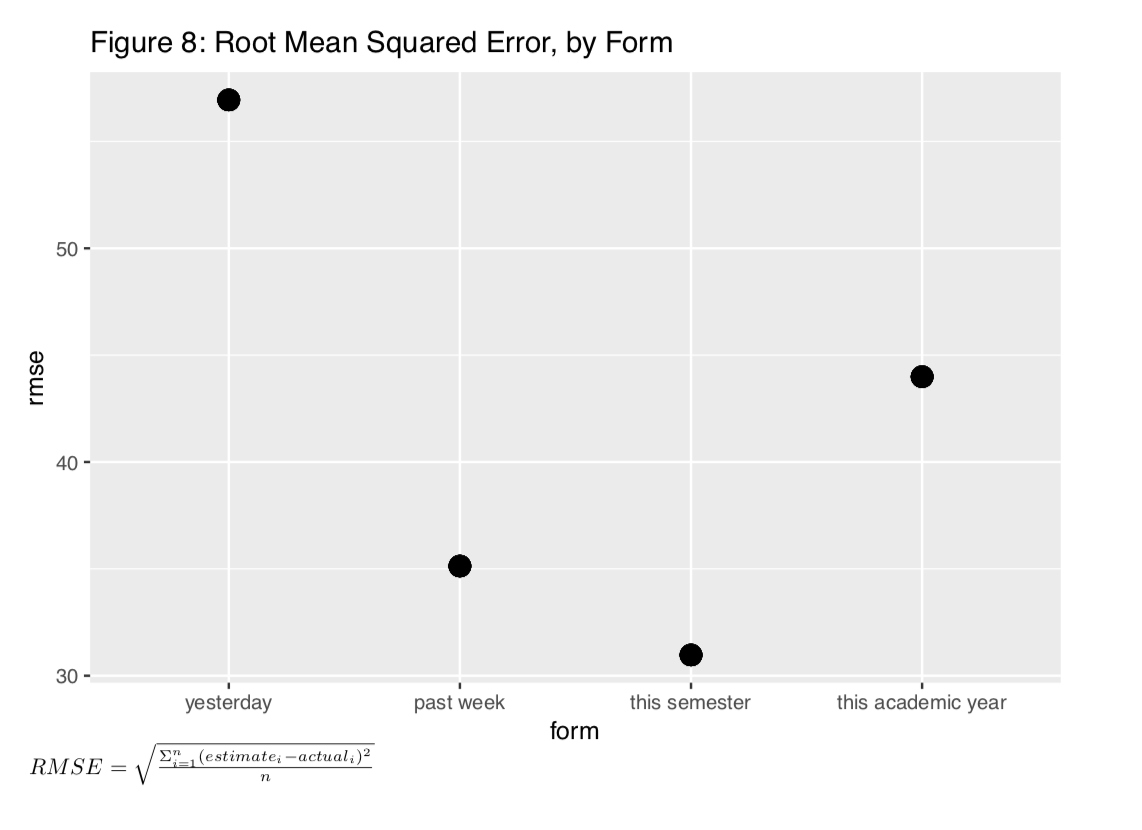
\includegraphics[width=0.7\textwidth]{figures/soc204_s2017_assignment8_mse_ushape}
\end{center}

\end{frame}
%%%%%%%%%%%%%%%%%%%%%%%%%%
\begin{frame}

\begin{center}
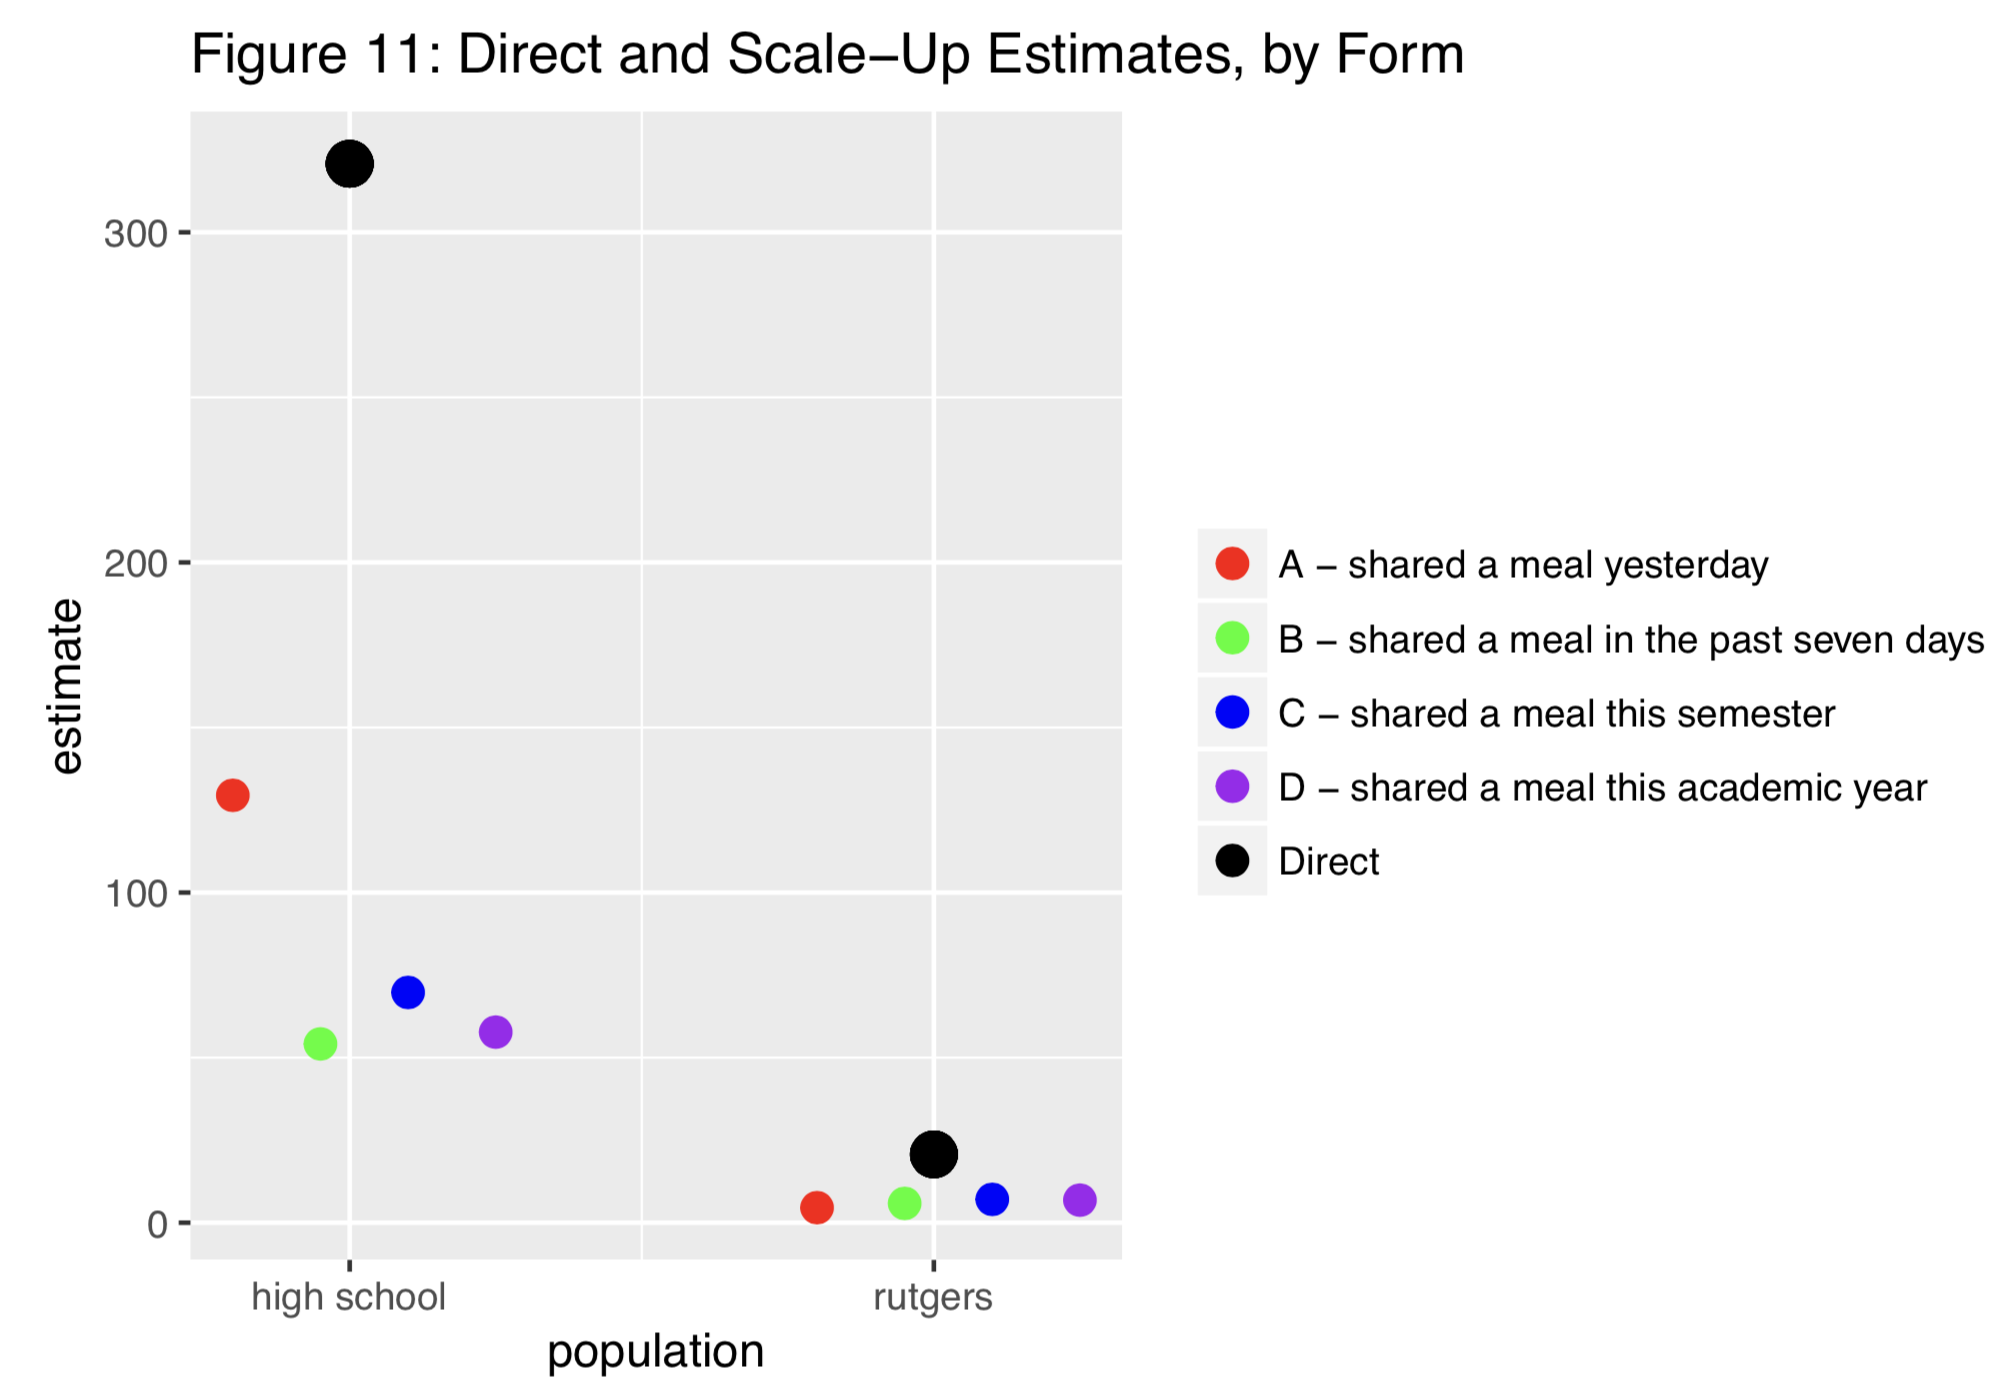
\includegraphics[width=0.7\textwidth]{figures/soc204_s2017_assignment8_estimates}
\end{center}

\begin{itemize}
\item scale-up estimates might be too low because of imperfect visibility
\end{itemize}


\end{frame}
%%%%%%%%%%%%%%%%%%%%%%%%%%
\begin{frame}

Lecture 23: Who knows what about who?
\begin{itemize}
\item Salganik, M.J. et al. (2011). The game of contacts: Estimating the social visibility of groups. \textit{Social Networks}.
\item Cowan, S. (2014). Secrets and Misperceptions: The Creation of Self-Fulfilling Illusions. \textit{Sociological Science}.
\end{itemize}

\end{frame}
%%%%%%%%%%%%%%%%%%%%%%%%%%


\end{document}
